\documentclass{article}
\usepackage[utf8]{inputenc}

\title{EE2703 Applied Programming Lab \\ Assignment 4}
\author{
  \textbf{Name}: Neham Hitesh Jain\\
  \textbf{Roll Number}: EE19B084
}\date{March 9, 2021}

\usepackage{listings}
\usepackage{natbib}
\usepackage{amsmath}
\usepackage{color}
\usepackage{graphicx}
\definecolor{dkgreen}{rgb}{0,0.6,0}
\definecolor{gray}{rgb}{0.5,0.5,0.5}
\definecolor{mauve}{rgb}{0.58,0,0.82}

\lstset{frame=tb,
  language=Python,
  aboveskip=3mm,
  belowskip=3mm,
  showstringspaces=false,
  columns=flexible,
  basicstyle={\small\ttfamily},
  numbers=none,
  numberstyle=\tiny\color{gray},
  keywordstyle=\color{blue},
  commentstyle=\color{dkgreen},
  stringstyle=\color{mauve},
  breaklines=true,
  breakatwhitespace=true,
  tabsize=3
}
\begin{document}

\maketitle
\newpage

\section{Introduction}


In this assignment we study the fourier series approximations of $e^x$ and $cos(cos(x))$. We first
compute the fourier series coefficients using the expression of sum of scaled harmonics. The
coefficients of the harmonics are computed using numerical integration provided by quad()
function in scipy. We then study another method for calculating fourier coefficients using least
square estimation.We further study the outcomes of the two mentioned methods and analyse
the results and cause of divergence.

\section{Fourier Series representation}


The Fourier Series representation of a function is basically an infinite series, whose each term is a complex constant (called coefficient) multiplied by a complex exponential. This can be equivalently converted into a series of cosines and sines.
\newline
\newline
\noindent
The Fourier Series of a function $f(x)$ with period $2\pi$ is computed as follows:
\begin{equation}
    f(x) = a_0 + \sum_{n=1}^{+\infty}\{ a_ncos(nx) +b_nsin(nx)\}
\end{equation}
\newline
where, 

\begin{equation}
    a_0 = \frac{1}{2\pi} \int_0^{2\pi}f(x)dx\\
\end{equation}
\begin{equation}
    a_n = \frac{1}{\pi} \int_0^{2\pi}f(x)*\cos(nx)dx
\end{equation}
\begin{equation}
    b_n = \frac{1}{\pi} \int_0^{2\pi}f(x)*\sin(nx)dx\\
\end{equation}
    
 For a function to have a Fourier Series representation, it must be periodic. f(x) = cos(cos(x)) is periodic but $e^x$ is not. So we deal with the periodic extension of $e^x$, with period $2\pi$, function extended from [0, $2\pi$] to [-$\infty$, +$\infty$].

\section{Plotting the functions}

We plot the function $e^x$ in log scale (both pure function as well as periodic extension). The following python snippets are used to declare the functions $e^x$ and cos(cos(x)). The x values range from -2${\pi}$ to 4${\pi}$.
The graph in Figure-1 shows the function $e^x$ on a log scale: both as an aperiodic exponential and a periodically extended exponential. The graph in Figure-2 shows the function $cos(cos(x))$ on an absolute scale. We can
clearly see its periodicity.

\begin{lstlisting}
def exponential(x):
    return np.exp(x)    

def cos_cos(x):
    return np.cos(np.cos(x))

def exp_extension(x):
    time_period=2*np.pi  
    return exponential(x%time_period)
    
def general_func_plot(x_vals,y_vals,title,fmt,type,xlabel,ylabel):
    plt.figure()
    plt.grid(True)
    if type =="semilogy":
        plt.semilogy(x_vals,y_vals,fmt)
    elif type =='log':
        plt.loglog(x_vals,y_vals,fmt)
    elif type =="normal_scale":
        plt.plot(x_vals,y_vals,fmt)
    plt.xlabel(xlabel)
    plt.ylabel(ylabel)
    plt.title(title)
    plt.savefig(f"plots/{title}.jpg")
\end{lstlisting}

\begin{figure}[!tbh]
    \centering
    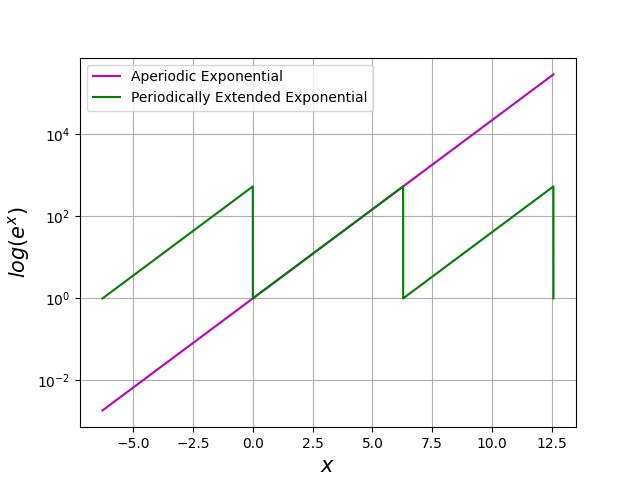
\includegraphics[scale=0.65]{plots/exponential.jpg}
    \caption{$e^x$}
    \label{fig:Figure 1}
    \end{figure}
    

\begin{figure}[!tbh]
    \centering
    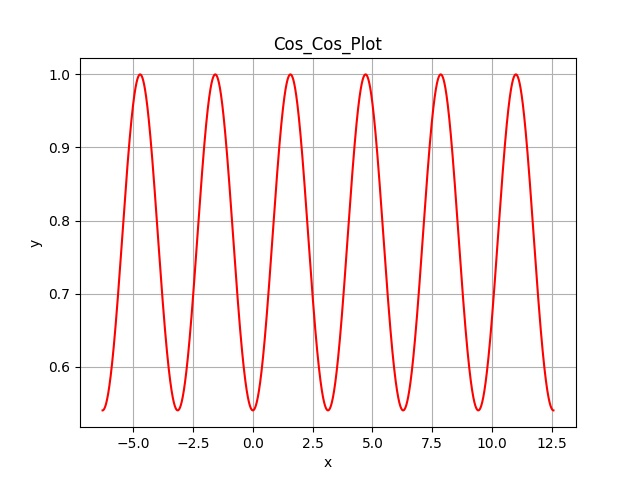
\includegraphics[scale=0.65]{plots/Cos_Cos_Plot.jpg}
    \caption{$cos(cos(x))$}
    \label{fig:Figure 2}
    \end{figure}
    


\hfill \break

To answer the questions posed in the assignment in this section, $cos(cos(x))$ is periodic with fundamental period $\pi$ (but here, for the Fourier Series Coefficient calculation I have taken the period $2\pi$, not that it matters a lot), $e^x$ is aperiodic and we have extended it to be periodic with period $2\pi$.

\section{Fourier Series Coefficients Calculation}


\par We create two new functions to be integrated, namely \begin{verbatim}
    def mul_by_cos(x,func,k):
        return func(x)*np.cos(k*x)
\end{verbatim} and
\begin{verbatim}
    def mul_by_sin(x,func,k):
        return func(x)*np.sin(k*x)
\end{verbatim}
We obtain the first 25 co-efficients for both $e^x$ and $cos(cos(x))$ by using the equations given in the introduction, scipy’s built in integrator, the quad function to pass extra arguments to the function being integrated. They are stored in a vector in the order
\begin{center}
     $
    \begin{pmatrix}
    a_0\\
    a_1\\
    b_1\\
    ...\\
    a25\\
    b25\\
    \end{pmatrix}
     $
    
\end{center}


\begin{lstlisting}

def calculate_fourier_series_coefffs(n,function):
    a = np.zeros(n)
    a[0] = scipy.integrate.quad(function,0,2*math.pi)[0]/(2*math.pi)
    for i in range(1,n):
        if(i%2==1):
            a[i] = scipy.integrate.quad(mul_by_cos,0,2*math.pi,args=(function,int(i/2)+1))[0]/math.pi
        else:
            a[i] = scipy.integrate.quad(mul_by_sin,0,2*math.pi,args=(function,int(i/2)+1))[0]/math.pi
    return a

\end{lstlisting}

 The first 51 fourier coefficients are plotted on different scales mainly semilog and loglog so as to analyse the decay of the coefficients.


\begin{figure}[!tbh]
    \centering
    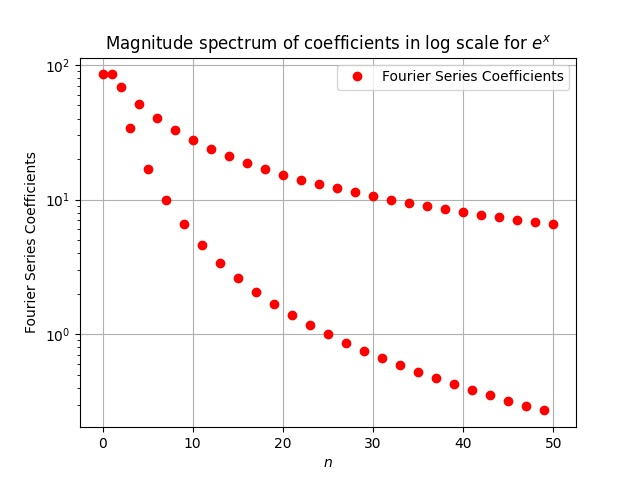
\includegraphics[scale=0.65]{plots/Magnitude spectrum of coefficients in log scale for $e^x$.jpg}
    \caption{Fourier Coefficients for $e^x$ in semilogy scale}
    \label{fig:Figure 3}
    \end{figure}

\begin{figure}[!tbh]
    \centering
    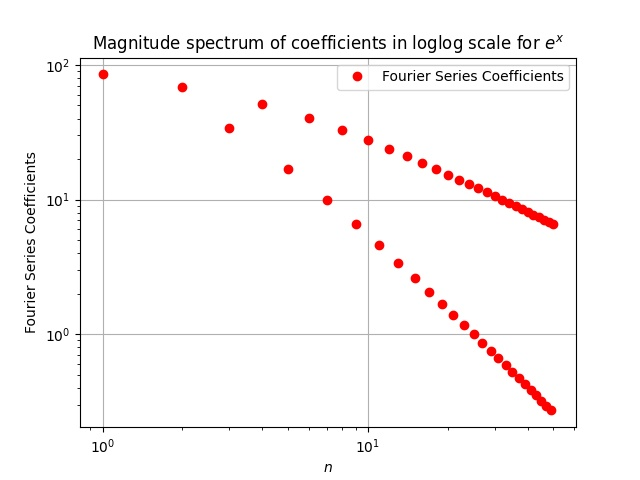
\includegraphics[scale=0.65]{plots/Magnitude spectrum of coefficients in loglog scale for $e^x$.jpg}
    \caption{Fourier Coefficients for $e^x$ in loglog scale}
    \label{fig:Figure 4}
    \end{figure}

\begin{figure}[!tbh]
    \centering
    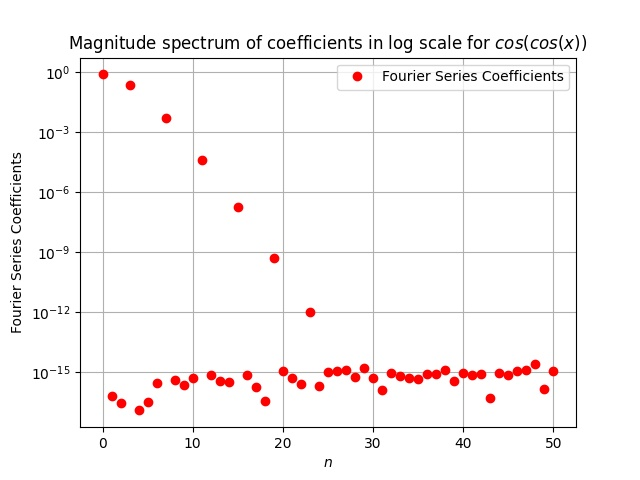
\includegraphics[scale=0.65]{plots/Magnitude spectrum of coefficients in log scale for $cos(cos(x))$.jpg}
    \caption{Fourier Coefficients for $cos(cos(x))$ in semilogy scale}
    \label{fig:Figure 5}
    \end{figure}

\begin{figure}[!tbh]
    \centering
    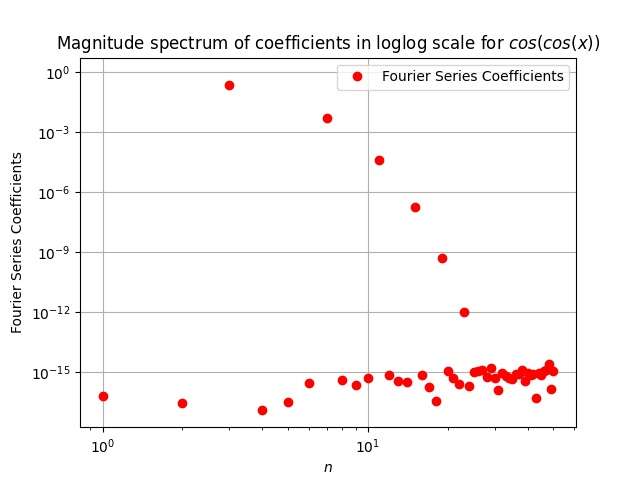
\includegraphics[scale=0.65]{plots/Magnitude spectrum of coefficients in loglog scale for $cos(cos(x))$.jpg}
    \caption{Fourier Coefficients for $cos(cos(x))$ in loglog scale}
    \label{fig:Figure 6}
    \end{figure}

 
\hfill \break
\hfill \break

\section{Observations}
\textbf{Q :} If you did Q.1 correctly, the $b_n$ coefficients in the second case should be nearly zero. Why does this happen?\newline
\textbf{A :} Yes. As we can see for cos(cos(x)), in both the log and loglog scale plots, the blue coloured dots which stand for $b_n$ have magnitude of the order of $10^{-16}$, which is vanishingly small. This happens because cos(cos(x)) is an even function, hence, theoretically speaking, its Fourier Series would be a pure cosine series with no sine terms (in other words, $b_k$ = 0 for all integers k). However, since Numpy evaluates integrals with numerical techniques, it is natural to not expect a 0 result from it. \newline \newline

\noindent\textbf{Q :} The coefficients for $cos(cos(x))$ decrease rapidly as compared to $e^x$ for higher frequencies. Why ?\newline
\textbf{A :} The function $e^x$ has many frequencies in it. So all its coefficients are non-zero and the decay is slow. On the contrary, cos(cos(x)) is a sinusoid type of function hence it has very less number of frequencies, which leads to quicker decaying coefficients.
\newline\newline

\noindent\textbf{Q :} Why does the loglog plot of Figure \ref{fig:Figure 5} look linear while the log plot of Figure \ref{fig:Figure 4} look linear ?\newline
\textbf{A :} The coefficients of $e^x$ decay with n as\\ \begin{center}
    $a_n \propto 1/n^2$\\ $b_n \propto 1/n$ 
\end{center} hence, taking log, $\log a_n$ and $\log b_n$ are almost proportional to log(n). So the loglog scale features linear behaviour. For cos(cos(x)) the FSC’s decay approximately exponentially with n i.e \begin{center}
    $a_n , b_n \propto e^{-n}$
\end{center}, and hence the log plot looks linear.

\section{Least Squares Aprroach}

We now obtain the fourier coefficients using another method ie: Least square approach. In this
method we solve the following equation by using least sqaure estimation


\[
\quad
\begin{pmatrix} 
1 & \cos(x_1) & \sin(x_1) & .... & \cos(25x_1) & \sin(25x_1)\\
1 & \cos(x_2) & \sin(x_2) & .... & \cos(25x_2) & \sin(25x_2)\\
... & ... & ... & .... & ... & ... \\
1 & \cos(x_{400}) & \sin(x_{400}) & .... & \cos(25x_{400}) & \sin(25x_{400})
\end{pmatrix}
\quad
\begin{pmatrix} 
a_0\\
a_1\\
b_1\\
...\\
a_{25}\\
b_{25}
\end{pmatrix}
=
\quad
\begin{pmatrix} 
f(x_1)\\
f(x_2)\\
...\\
f(x_{400})
\end{pmatrix}
\]
\\Here, the values $x_1$ to $x_{400}$ are chosen uniformly from 0 to $2\pi$. We would carry out our regular procedure of using lstsq to find the column matrix of coefficients which best fits the equation. 

\par The below shown graphs show the difference in values of coefficients calculated using the two methods.


\begin{lstlisting}
#Least Squares Approach
x = np.linspace(0,2*np.pi,401)
x=x[:-1]  
A = np.zeros((400,51)) 
A[:,0]=1 
for k in range(1,26):
    A[:,2*k-1] = np.cos(k*x) 
    A[:,2*k] = np.sin(k*x) 
#Matrix A (51 x 400) has been defined 

coeffs_exp_lstsq = matrix_method(A,exponential,x)       #Calling above function
coeffs_cos_cos_lstsq = matrix_method(A,cos_cos,x) 

def comparing_coeffs(coeffs_int,coeffs_mat,type,xlabel,title,ylabel):
    plt.figure()
    if type=="semilogy":
        plt.semilogy(np.abs(coeffs_int),'go',label=r'Integration Approach')
        plt.semilogy(np.abs(coeffs_mat),'bo',label=r"Least Squares Approach")
    if type=="loglog":
        plt.loglog(np.abs(coeffs_int),'go',label=r'Integration Approach')
        plt.loglog(np.abs(coeffs_mat),'bo',label=r'Least Squares Approach')
    plt.legend()
    plt.grid(True)
    plt.title(title)
    plt.ylabel(xlabel)
    plt.xlabel(ylabel)
    plt.savefig(f"plots/{title}.jpg")

\end{lstlisting}

\hfill \break
The following plots display the FSC's obtained by Integration and Least Squares approach in log and loglog scales.

\begin{figure}[!tbh]
    \centering
    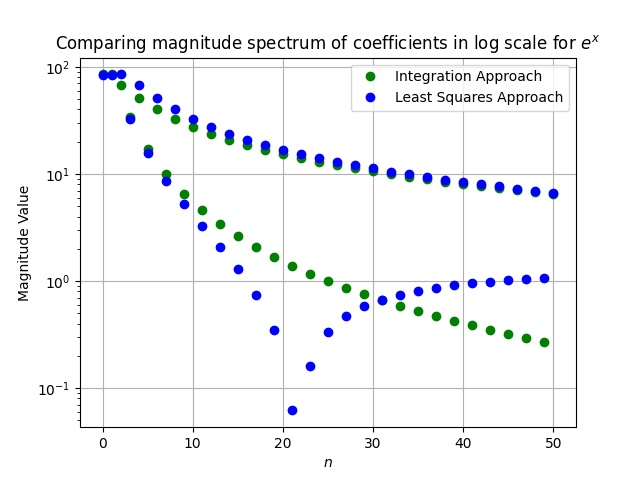
\includegraphics[scale=0.65]{plots/Comparing magnitude spectrum of coefficients in log scale for $e^x$.jpg}
    \caption{Comparing Fourier Coefficients for $e^x$ in log scale}
    \label{fig:Figure 7}
    \end{figure}

\begin{figure}[!tbh]
    \centering
    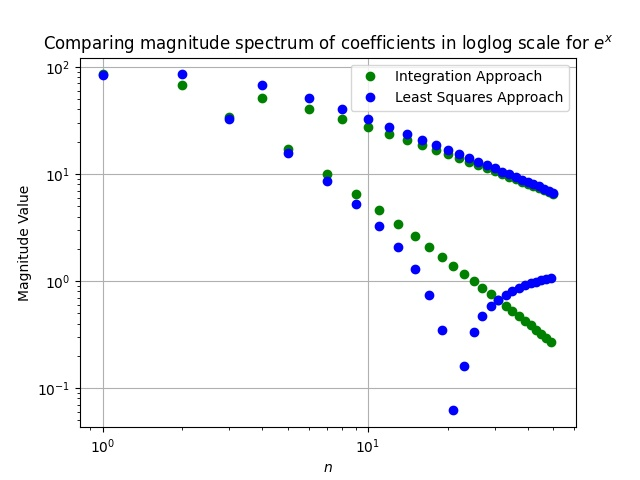
\includegraphics[scale=0.65]{plots/Comparing magnitude spectrum of coefficients in loglog scale for $e^x$.jpg}
    \caption{Comparing Fourier Coefficients for $e^x$ in loglog scale}
    \label{fig:Figure 8}
    \end{figure}

\begin{figure}[!tbh]
    \centering
    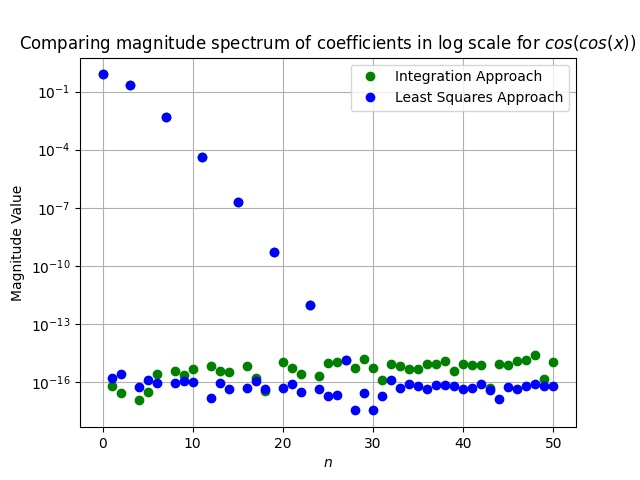
\includegraphics[scale=0.65]{plots/Comparing magnitude spectrum of coefficients in log scale for $cos(cos(x))$.jpg}
    \caption{Comparing Fourier Coefficients for $cos(cos(x))$ in log scale}
    \label{fig:Figure 9}
    \end{figure}

\begin{figure}[!tbh]
    \centering
    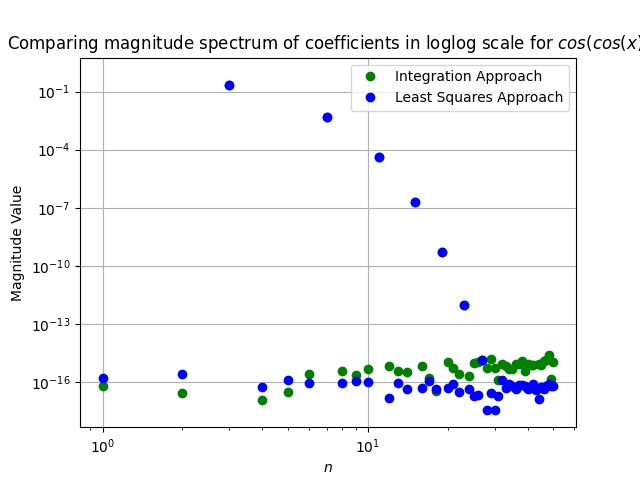
\includegraphics[scale=0.65]{plots/Comparing magnitude spectrum of coefficients in loglog scale for $cos(cos(x))$.jpg}
    \caption{Comparing Fourier Coefficients for $cos(cos(x))$ in loglog scale}
    \label{fig:Figure 10}
    \end{figure}

\hfill \break
\hfill \break

\section{Analysing the deviation}

It was found that the maximum error in values of coefficients (obtained by both methods) of $e^x$ was 17.32221313 and the same for cos(cos(x)) was $2.67 x 10^{-15}$

\section{Convergence of Fourier Series representation to actual function}

Now, using the values of coefficients obtained from the direct Integration method, we reconstruct the function by multiplying by the sinusoids (in short, multiply those 2 matrices in the LHS to get a list of function values that will approximate function behaviour)

\begin{lstlisting}
fourier_func_exp = np.matmul(A,coeffs_exp_lstsq)
fourier_func_cos = np.matmul(A,coeffs_cos_cos_lstsq)
def plotting_convergence(fourier_func,f,x_vals,title,xlabel,ylabel):            
    plt.figure()
    plt.semilogy(fourier_func, 'm', label = 'Fourier representation')
    plt.semilogy(f(x_vals), 'c', label = 'Original function')
    plt.grid(True)
    plt.legend(loc='upper right')
    plt.title(title)
    plt.ylabel(xlabel)
    plt.xlabel(ylabel)
    plt.savefig(f"plots/{title}.jpg")  

\end{lstlisting}

\begin{figure}[!tbh]
    \centering
    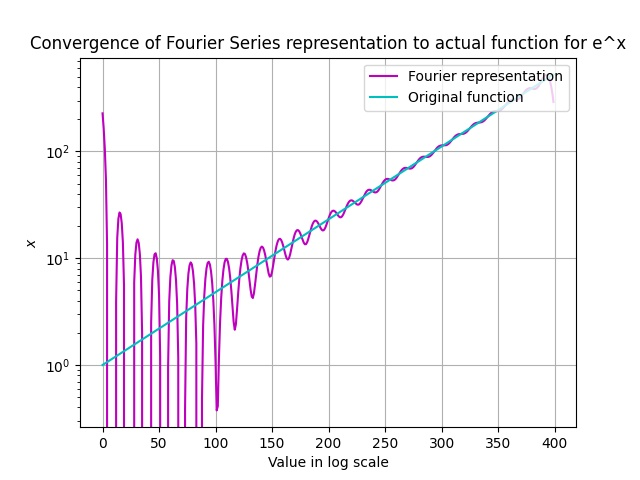
\includegraphics[scale=0.7]{plots/Convergence of Fourier Series representation to actual function for e^x.jpg}
    \caption{Actual and predicted values for $e^x$}
    \label{fig:Figure 11}

    \end{figure}

\begin{figure}[!tbh]
    \centering
    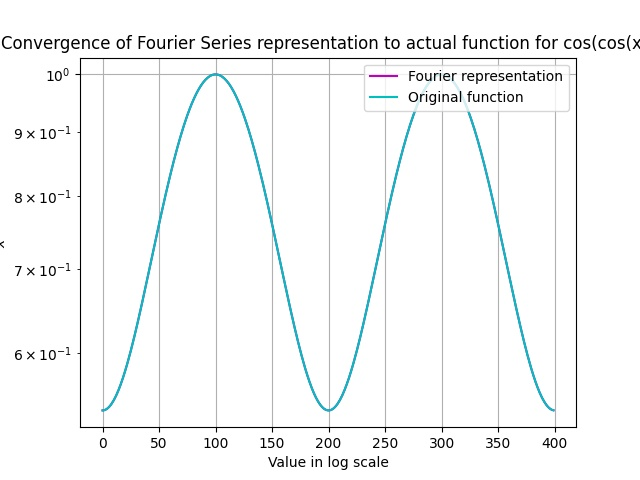
\includegraphics[scale=0.7]{plots/Convergence of Fourier Series representation to actual function for cos(cos(x)).jpg}
    \caption{Actual and predicted values for $cos(cos(x))$}
    \label{fig:Figure 12}

    \end{figure}


\hfill \break
\hfill \break

The Fourier Series representation thus obtained converges stunningly well for y = cos(cos(x)) but poorly for $e^x$. 
\newline \newline
The Gibbs phenomenon is an overshoot (or ”ringing”) of Fourier series and other eigenfunction series occurring at simple discontinuities. The partial sums of the Fourier series will have large oscillations near the discontinuity of the function. 
\newline \newline
These oscillations do not die out as n increases, but approaches a finite limit.. Just as an instance, y = cos(x) just needs one FSC and this will perfectly represent it. But we see that even 51 FSC's fall short of representing $e^x$ decently.

\newpage
\section{Conclusion}

\par In this assignment, we learnt how to calculate the fourier series coefficients for a perodic function by two methods, namely integration and least square.
\newline \newline
Also, we saw that as our $e^x$ was discontinuous, there was significant error between the curve we predicted and the actual curve. Whereas that was not the case for $cos(cos(x))$. This discontinuity leads to non uniform convergence of the Fourier series, which means that the partial sums obtained using the fourier coefficients converge at different rates for different values of x.
\newline \newline
This difference in the rates of convergence leads to the property of Gibb’s phenomenon, which is the observed at discontinuities in the Fourier estimation of a discontinuous function. This oscillation is present for any finite N, but as N → ${\infty}$ the series begins to converge. This explains the mismatch in the Fourier approximation for $e^x$ .
\end{document}
